
\documentclass[12pt]{article}
\usepackage[T1]{fontenc}
% \usepackage{babel}
\usepackage{titling}
\usepackage{blindtext}
\usepackage{geometry}
\usepackage{hyperref}

\usepackage{epsfig}
\usepackage{graphicx}


\setlength{\droptitle}{-6em}     % Eliminate the default vertical space
\addtolength{\droptitle}{-4pt}   % Only a guess. Use this for adjustment

\title{\Large \bf 2.152 Project: \\ Adaptive Control of 2-Link Robotic Arm}
\author{\vspace{-6em}Luke Roberto}
\date{\vspace{-6em}May 14th, 2018}
\maketitle

\begin{document}

\vspace{-2em}

%%%%%%%%%%%%%%%%%%%%%%%%%%%%%%%%%%%%%%%%%%%%%%%%%%%%%%%%%%%%%%%%%%%%%%%%%%%%%%%%%%%%%%%%
\section{Setup}

The purpose of this project was to implement composite adaptive control on an interesting system while also learning to use the Julia programming language. The project code is located at: \url{https://github.com/Lukeroberto/2.152_project}. There are a collection of Julia Notebooks that can be viewed without actually installing the language on your system, you can also view short gifs of the results as well.
\\

%%%%%%%%%%%%%%%%%%%%%%%%%%%%%%%%%%%%%%%%%%%%%%%%%%%%%%%%%%%%%%%%%%%%%%%%%%%%%%%%%%%%%%%%
\section{Adaptive Control of Double Integrator}

The first steps of this project were to model a simple system. This allowed me a little time to get comfortable with the language and build intuition on how the adaptive controller worked realtime.
\\

\begin{figure}[h]
    \centering
    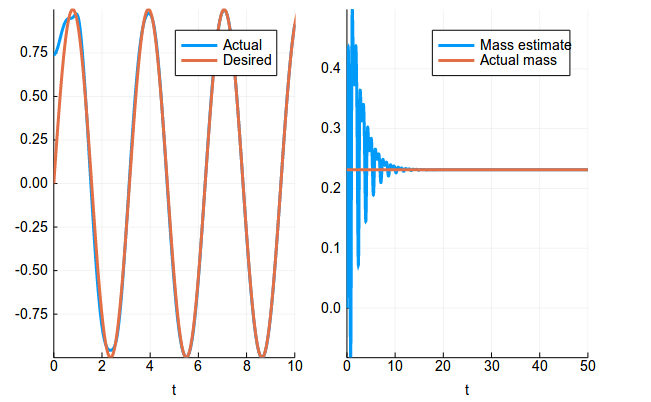
\includegraphics[width=3.5in\textsize]{double_integrator_adaptation.png}
    \caption{Tracking $sin(2t)$}
    \label{fig:double_integrator_sine}
\end{figure}

\noindent
The setup was easy to implement, the MRAC policy given in chapter 8, with control policy 8.3 and adaptation law 8.6, was used to track a number of trajectories. Fig.~\ref{fig:double_integrator_sine} shows the controller tracking $sin(2t)$. There is nice exponential convergence as expected, although intuitively it is interesting to me how the controller has essentially zeros error around $t=4$, yet does not learn the mass until approximately $t=15$. I assume the nature of the controller has a good deal of robustness, especially when the mass estimate error shrinks below a sufficient threshold.
\\

\begin{figure}[h]
    \centering
    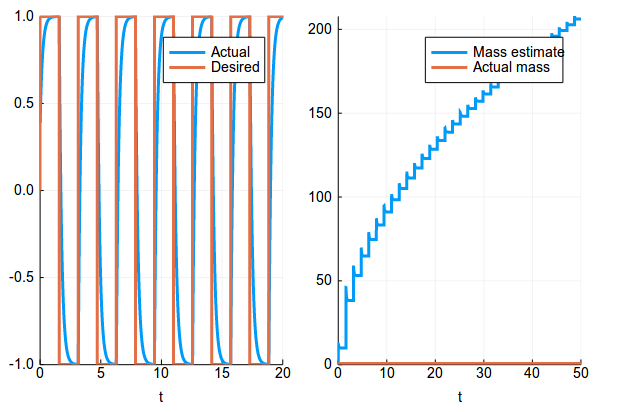
\includegraphics[width=3.5in\textsize]{double_integrator_square_wave.png}
    \caption{Tracking $sgn(sin(2t))$}
    \label{fig:double_integrator_sq}
\end{figure}

\noindent

After testing out the controller on a trivial set of trajectories, I decided to see what would happen if I were to break some of the assumptions that were made in the derivations of adaptive control. The most interesting one in my opinion is shown in Fig.~\ref{fig:double_integrator_sq}. The desired trajectory is not continuous and its derivatives are not even differentiable. The closed loop system acts behaves like a second order system trying to follow a square wave input, even though the mass estimate grows unbounded. This may be an artifact of the implementation, but an interesting observation nonetheless.
\\


%%%%%%%%%%%%%%%%%%%%%%%%%%%%%%%%%%%%%%%%%%%%%%%%%%%%%%%%%%%%%%%%%%%%%%%%%%%%%%%%%%%%%%%%
\section{Adaptive Control of 2-Link Arm}

Once I was able to test out the double integrator system, I then moved on to control of the 2-link arm dynamics as specified in example 9.1 of the textbook.

\begin{figure}[h]
    \centering
    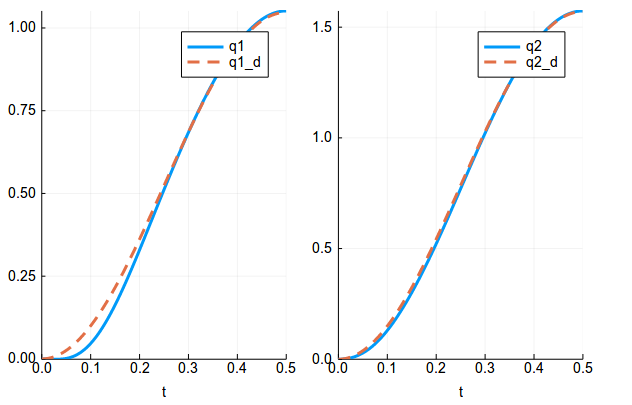
\includegraphics[width=3.5in\textsize]{arm_trajectory_tracking.png}
    \caption{Tracking $sgn(sin(2t))$}
    \label{fig:arm1}
\end{figure}


\begin{figure}[h]
    \centering
    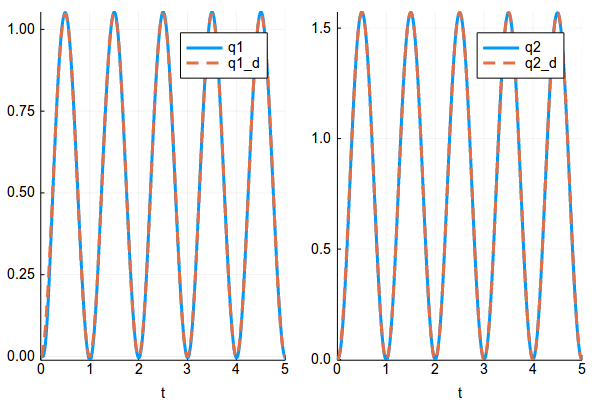
\includegraphics[width=3.5in\textsize]{arm_trajectory_tracking2.png}
    \caption{Tracking $sgn(sin(2t))$}
    \label{fig:arm2}
\end{figure}

\begin{figure}[h]
    \centering
    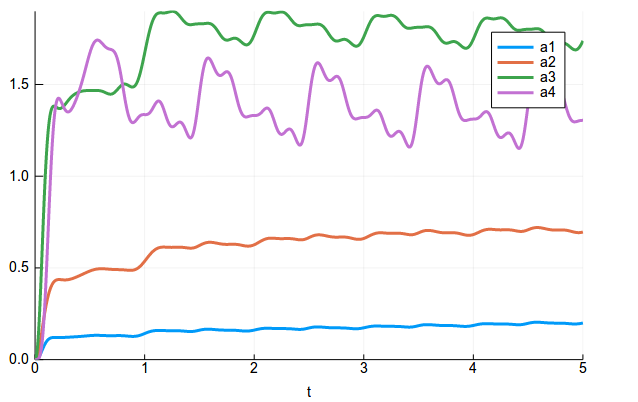
\includegraphics[width=3.5in\textsize]{arm_parameter_estimates.png}
    \caption{Tracking $sgn(sin(2t))$}
    \label{fig:arm_param}
\end{figure}

%%%%%%%%%%%%%%%%%%%%%%%%%%%%%%%%%%%%%%%%%%%%%%%%%%%%%%%%%%%%%%%%%%%%%%%%%%%%%%%%%%%%%%%%
\section{Composite Adaptive Control}



\end{document}
